%%%%%%%%%%%%%%%%%%%%%%%%%%%%%%%%%%%%%%%%%%%%%%%%%%%%%%%%%%%%%%%%%%%%%%
%%	Name: "Signal analysis template"
%%	File name: signalanalysis_template_main
%%	Version: 1.5
%%
%%	Compiler: XeLaTeX
%%
%%%%%%%%%%%%%%%%%%%%%%%%%%%%%%%%%%%%%%%%%%%%%%%%%%%%%%%%%%%%%%%%%%%%%%

\documentclass[conference,compsoc,onecolumn]{IEEEtran}

% *** LANGUAGE UTILITY PACKAGES ***
\usepackage[utf8]{inputenc} % Required for including letters with accents
\usepackage[spanish]{babel}
\usepackage{hyperref}
\usepackage{graphicx}
% *** USED PACKAGES ***
% *** MISC UTILITY PACKAGES ***
\usepackage{comment}			% Agregar comentarios
\usepackage{lipsum}				% Inserts dummy text
\usepackage{blindtext}
\usepackage{listings}					% Coding
\usepackage{verbatim}				% Verbatim
\usepackage[final]{pdfpages}
\usepackage{booktabs,dcolumn}
\usepackage{pdflscape}
\usepackage{afterpage}
%\setlist[itemize]{noitemsep, nolistsep}
\usepackage[bookmarks=false]{hyperref}
\usepackage{tcolorbox}									% Coloured boxes, for LATEX examples and theorems, etc
\usepackage{color}
\usepackage{xcolor} % Required for specifying colors by name									% Color packages foreground and back­ground color man­age­men
% *** CITATION PACKAGES ***
\usepackage{cite}
% *** GRAPHICS RELATED PACKAGES ***
\usepackage{graphicx}
\usepackage{caption}
\usepackage{pgfplots}
\usepackage{tikz}
\usetikzlibrary{shapes,arrows}
\usetikzlibrary{decorations.pathmorphing} % noisy shapes
\usetikzlibrary{fit}					% fitting shapes to coordinates
\usetikzlibrary{backgrounds}	% drawing the background after the foreground
\pgfplotsset{compat=1.13}
% *** MATH PACKAGES ***
\usepackage{amsmath}
\usepackage{mathtools}
\usepackage{amssymb}
\usepackage{amsfonts}
\usepackage{expl3}
\usepackage{bm}

% *** SPECIALIZED LIST PACKAGES ***
\usepackage{algorithmic}
\usepackage{listings}					% Coding
\usepackage[framed,numbered,autolinebreaks,useliterate]{mcode}
% *** ALIGNMENT PACKAGES ***
\usepackage{array}
% *** SUBFIGURE PACKAGES ***
%\ifCLASSOPTIONcompsoc
%\usepackage[caption=false,font=normalsize,labelfont=sf,textfont=sf]{subfig}
%\else
%\usepackage[caption=false,font=footnotesize]{subfig}
%\fi
% *** FLOAT PACKAGES ***
\usepackage{fixltx2e}
\usepackage{stfloats}
%\fnbelowfloat
%\usepackage{dblfloatfix}
% *** PDF, URL AND HYPERLINK PACKAGES ***
\usepackage{url}
\usepackage{everypage}


\usepackage{multirow} % In order to be able to insert rows spanning multiple lines
\usepackage{verbatim}
\usepackage[all]{xy}
\usepackage{listings}
\usepackage{subfigure}
\usepackage{multibib}
\usepackage{setspace} 
\usepackage{algorithm}			    	  % To insert nice algorithms

% *** CARPETA DONDE SE GUARDARAN LAS IMAGENES ***
\graphicspath{{figures/}}

% *** NUEVOS COMANDOS Y CONFIGURACIONES VARIAS ***
\interdisplaylinepenalty=2500
\newcommand{\Lpagenumber}{\ifdim\textwidth=\linewidth\else\bgroup
	\dimendef\margin=0
	\ifodd\value{page}\margin=\oddsidemargin
	\else\margin=\evensidemargin
	\fi
	\raisebox{\dimexpr -\topmargin-\headheight-\headsep-0.5\linewidth}[0pt][0pt]{%
		\rlap{\hspace{\dimexpr \margin+\textheight+\footskip}%
			\llap{\rotatebox{90}{\thepage}}}}%
	\egroup\fi}

\AddEverypageHook{\Lpagenumber}%

\newcommand{\newtxt}[1]{\textcolor{black}{#1}}
\renewcommand\IEEEkeywordsname{Palabras cláve:}
\newcommand{\mx}[1]{\mathbf{\bm{#1}}} % Matrix command
\newcommand{\vc}[1]{\mathbf{\bm{#1}}} % Vector command

%% Separación de palabras
\hyphenation{op-tical net-works semi-conduc-tor HHMMSS}


\begin{document}

% *** TITLES AND NAMES ***
% title of the document
\title{Proyecto de aula: Plataforma de seguimiento de datos COVID-19 para Colombia}
% author names and affiliations
\makeatletter
\newcommand{\linebreakand}{%
    \end{@IEEEauthorhaling}
    \hfill\mbox{}\par
    \mbox{}\hfill\begin{@IEEEauthorhalign}
}
\makeatother
%%%%
\author{\IEEEauthorblockN{Lady~Geraldine~Salazar~Bayona}
\IEEEauthorblockA{Escuela de Ciencias Exactas\\
Universidad Sergio Arboleda-Bogotá, Colombia\\
lady.salazar01@correo.usa.edu.co}
\and
\IEEEauthorblockN{Juan~Pablo~Mora~Aragón}
\IEEEauthorblockA{Escuela de Ciencias Exactas\\
Universidad Sergio Arboleda-Bogotá, Colombia\\
juan.mora03@correo.usa.edu.co}
\linebreakand
\IEEEauthorblockN{Jessica~Valentina~Parrado~Alfonso}
\IEEEauthorblockA{Escuela de Ciencias Exactas\\
Universidad Sergio Arboleda-Bogotá, Colombia\\
jessica.parrado01@correo.usa.edu.co}}

% *** MAKE TITLE ***
\maketitle
\IEEEoverridecommandlockouts
\IEEEpeerreviewmaketitle

\begin{abstract}
En el presente laboratorio se aplicarán los procesos necesarios para extraer información de páginas web con datos actualizados sobre la pandemia actual que ha cambiado al mundo, esto se hará usando el lenguaje de programación interpretado Python el cual permite de manera sencilla la extracción, interpretación y la realización de las gráficas. Es de destacar que para el proceso de adquirir la información se hace necesario una amplia investigación para poder hallar la base de datos adecuada. Todo lo anterior se elaboró con el objetivo de informar mediante graficas de dos dimensiones la situación actual por la que pasa la humanidad en esta pandemia. Los resultados y el proceso se podrán visualizar a lo largo del proyecto detalladamente.
\end{abstract}


\begin{IEEEkeywords}
    \LaTeX, PDF, Proyecto, Análisis de datos, Gráficas, Python, Pandas, WebScraping, Pandemia.
\end{IEEEkeywords}


\section{Marco teórico}
\label{sec:introduction}

\textbf{Pandemia actual Covid-19.}
\\\

\justify
\\\

COVID‑19 es la enfermedad infecciosa causada por el coronavirus que se ha descubierto más recientemente. Tanto este nuevo virus como la enfermedad que provoca eran desconocidos antes de que estallara el brote en Wuhan (China) en diciembre de 2019. Actualmente la COVID‑19 es una pandemia que afecta a muchos países de todo el mundo entre esos Colombia.
\\\

\justify
\\\
El ministro Fernando Ruiz destacó que la situación del contexto mundial sirve para entender la de Colombia. "En nuestro país tuvimos la misma situación, casi que cuatro capítulos diferentes. Un primer momento en Leticia, que no fue una epidemia colombiana sino brasilera -es decir la afectación de Leticia es más parecida a la de Brasil que a la de Colombia-, muy rápida, alta y un impacto altísimo", explicó.
\\\

\justify
\\\
Por lo pronto, se destaca la estrategia de Colombia y que ha sido referente a nivel mundial, buscando siempre aplanar la curva con la implicación de extender la epidemia un poco. "Hacerla más prolongada, de menor impacto, buscando una mayor inmunidad en la población, entonces digamos que la apuesta ha sido esa".
\\\

\justify
\\\
Estas medidas se tomaron con el conocimiento de lo que paso en Europa, con Italia y España principalmente. De ahí en adelante Colombia ha venido tomando decisiones que ya comprenden tres fases y aperturas graduales, que, si se comparan con las de otros países de la región, nuestro país lo ha hecho bien, ya que no ha habido la necesidad de retroceder. .~\cite{1}
\\\

\justify
\\\
El último informe del Ministerio de Salud y Protección Social, entregado el martes 29 de septiembre, confirmó 5.839 nuevos casos, 187 fallecidos más para un total de 25.828, mientras que 734.154 pacientes se han recuperado..~\cite{2}
\\\

\textbf{Python}
\\\

Python es un lenguaje de programación interpretado de tipado dinámico Se trata de un lenguaje de programación creado en 1991 por Guindo Van Rossum (1956, Holanda). Python es una opción interesante para realizar todo tipo de programas que se ejecuten en cualquier máquina. Está orientado a objetos y preparado para realizar cualquier tipo de programa, con este lenguaje podemos desarrollar software para app científicas, para comunicaciones de red, para app de escritorio con interfaz gráfica de usuario (GUI), para crear videojuegos, para smartphones, para inteligencia artificial, para automatización de tareas y por supuesto, para programación web..~\cite{3}
\\\

Para realizar este proyecto es necesario importar los siguientes paquetes:
\\\

\begin{itemize}
\item import pandas as pd: Pandas es una librería de python destinada al análisis de datos, que proporciona unas estructuras de datos flexibles y que permiten trabajar con ellos de forma muy eficiente. Pandas ofrece las siguientes estructuras de datos. Es necesario instalarlo previamente, el comando es: pip install pandas.~\cite{4}
\item import matplotlib.pyplot as plt: Matplotlib es probablemente el paquete de Python más utilizado para gráficos 2D. Proporciona una manera muy rápida de visualizar datos y figuras con calidad de publicación en varios formatos. Vamos a explorar Matplotlib en modo interactivo cubriendo los casos más comunes. Es necesario instalarlo previamente, el comando es pip install matplotlib..~\cite{5}
\item import os: El módulo os de Python le permite a usted realizar operaciones dependientes del Sistema Operativo como crear una carpeta, listar contenidos de una carpeta, conocer acerca de un proceso, finalizar un proceso, etc. Este módulo tiene métodos para ver variables de entornos del Sistema Operativo. Es necesario instalarlo previamente, el comando es: pip install os-sys..~\cite{6}
\item import requests: requests es una librería Python que facilita enormemente el trabajo con peticiones HTTP. Antes o después, en algún proyecto, es posible que tengas que hacer peticiones web, ya sea para consumir un API, extraer información de una página o enviar el contenido de un formulario de manera automatizada. Es necesario instalarlo previamente, el comando es: pip install requests.~\cite{7}
\end{itemize}
\\\

\textbf{EXTRACCIÓN DE DATOS}
\\\

Para lograr un uso adecuado de la información para los fines propuestos, primero tenemos que saber la forma de extraer datos, organizarlos, para luego poder trabajar con ellos.
\\\

 \textsl{CSV}: Un csv (comma-separated values) es un archivo de texto que almacena los datos en forma de columnas, separadas por coma y las filas se distinguen por saltos de línea.
 \\\
 
 Normalmente para importar o exportar de bases de datos de unas aplicaciones. Los programas de hojas de cálculo más habituales te dan la opción de grabar tu archivos en este formato, con la opción de  \textsl{“guardar como”}.~\cite{8}
 \\\

\textbf{WebScraping}
\\\

El web scraping consiste en navegar automáticamente una web y extraer de ella información. Esto puede ser muy útil para muchísimas cosas y beneficioso para casi cualquier negocio. A día de hoy, no creo que exista una sola empresa de éxito que no lo haga —o que no quiera hacerlo—. De hecho, la empresa reina del scrapeo es Google, que para que su buscador funcione así de bien tiene que estar constantemente scrapeando la red entera.
\\\

Al software programado para scrapear se le suele llamar bot, spider o crawler. Todo el mundo puede programar un crawler, ya que existen herramientas para ponerlo a punto que no requieren conocimientos de programación. Eso sí, estas herramientas nunca te van a dar toda la flexibilidad que tendrías si los desarrollaras en un lenguaje de programación. Más adelante veremos las tecnologías y herramientas más utilizadas para la creación de estos bichitos.~\cite{9}
\\\

\textbf{PANDAS}
\\\

Pandas es un paquete de Python que proporciona estructuras de datos similares a los dataframes de R. Pandas depende de Numpy, la librería que añade un potente tipo matricial a Python. Los principales tipos de datos que pueden representarse con pandas son:
\\\

\begin{itemize}
\item Datos tabulares con columnas de tipo heterogéneo con etiquetas en columnas y filas.
\item Series temporales.~\cite{10}
\end{itemize}
\\\

\\\
\section{Resultados}
\label{sec:results}

Para la realización de este proyecto se utilizó el siguiente código:
\\\

Primero se deben importar las librerías necesarias para la ejecución correcta del programa:
\\\

\begin{lstlisting}
import csv
import os
import urllib
import requests
import pandas as pd
import datetime
import matplotlib.pyplot as plt
import numpy as np
import plotly.express as px
import plotly

\end{lstlisting}
\\\
Luego, se utiliza el siguiente código para ingresar al sitio web en donde están los datos necesarios para el proyecto (tanto de Bogotá y Colombia) y así poder descargar de manera local los archivos CSV con todos los datos.\\\

\begin{lstlisting}
#Ingresar al sitio y descargar el CSV con los datos de Colombia
url="https://www.datos.gov.co/api/views/gt2j-8ykr/rows.csv?accessType=DOWNLOAD&bom=true&format=true"
response = requests.get(url)
with open(os.path.join("Archivo", "DataColombia.csv"), "wb") as f:
    f.write(response.content)

#Ingresar al sitio y descargar el CSV con los datos de Bogotá
url="https://datosabiertos.bogota.gov.co/dataset/44eacdb7-a535-45ed-be03-16dbbea6f6da/resource/b64b...
a3c4-9e41-41b8-b3fd-2da21d627558/download/osb_enftransm-covid26102020.csv"
response = requests.get(url)
with open(os.path.join("Archivo", "DataBogota.csv"), "wb") as f:
    f.write(response.content)

\end{lstlisting}
\\\

\textbf{CÓDIGO PARA DATOS COVID COLOMBIA}
\\\

Para el caso de Colombia  se abre el archivo CSV local y se obtienen todos los datos. Además, se hace el arreglo de los nombres de las columnas y se establece que para la columna del "Sexo" de la persona debe ser "M" o "F".
\\\
\begin{lstlisting}
#///////////////////COLOMBIA///////////////////////////////////////
#Abrir el CSV que se descargó de Colombia y obtener la información

data =pd.read_csv('Archivo/DataColombia.csv')


data.head()

data.columns=['Fecha', 'ID', 'Fecha2', 'Código DIVIPOLA', 'Departamento', 'Código DIVIPOLA2', 'Ciudad','Edad','Unnidad', 'Sexo', 'Tipo', 'Ubicacion','Atencion', 'Código ISO del país','Nombre del país','Recuperado','Fecha de inicio de síntomas','Fecha de muerte','Fecha de diagnóstico','Fecha de recuperación','Tipo de recuperación','Pertenencia étnica','Nombre del grupo étnico']

d={'m':'M', 'f':'F','F':'F', 'M':'M'}
data['Sexo']=data['Sexo'].apply(lambda x:d[x])

data['Fecha'] = pd.to_datetime(data['Fecha'])
\end{lstlisting}
\\\

Después se realiza el código para crear las 4 gráficas de Barras y las 2 gráficas de Tortas, en donde se busca representar los datos sobre los Departamentos, Sexo, Recuperados, Fallecido y según su condición.
\\\

\begin{lstlisting}
#GRÁFICAS DE BARRAS

fig1=plt.figure(figsize=(12,6))
data.Departamento.value_counts().plot(kind='bar', alpha=0.5)
plt.title('Número de Casos Totales según Departamento en Colombia')
plt.show()

fig=plt.figure(figsize=(12,6))
data.Sexo.value_counts().plot(kind='bar', alpha=0.5)
plt.title('Número de Casos totales en Colombia según el Sexo')
plt.show()

fig2=plt.figure(figsize=(12,6))
data.Recuperado[data.Recuperado == "Recuperado"].value_counts().plot(kind='bar', alpha=0.5)
plt.title('Número de Casos de Recuperados en Colombia')
plt.show()

fig3=plt.figure(figsize=(12,6))
data.Recuperado[data.Recuperado == "Fallecido"].value_counts().plot(kind='bar', alpha=0.5)
plt.title('Número de Casos de Fallecidos en Colombia')
plt.show()

#GRÁFICAS DE TORTAS

fig1=plt.figure(figsize=(12,6))
plt.pie(data.Sexo.value_counts(), autopct="%1.1f%%", shadow=True, radius= .9)
plt.title('Porcentaje de Casos totales en Colombia según el Sexo', bbox={"facecolor":"0.8","pad":5})
plt.legend( labels= data.Sexo.value_counts().index.unique(), loc='upper right')
plt.show()

fig1=plt.figure(figsize=(12,6))
plt.pie(data.Recuperado[data.Recuperado != "fallecido"].value_counts(), autopct="%1.1f%%", shadow=True, radius= .999)
plt.title('Porcentaje de la situación de los contagiados en Colombia', bbox={"facecolor":"0.8","pad":5})
plt.legend( labels=data.Recuperado.value_counts().index.unique(), loc='upper right')
plt.show()

\end{lstlisting}
\\\

Al ejecutar todo el código se obtienen las siguientes gráficas:
\\\

\begin{figure}[htbp]
\centering
\subfigure[\scriptsize Gráfica Número de Casos Totales según el Departamento en Colombia]{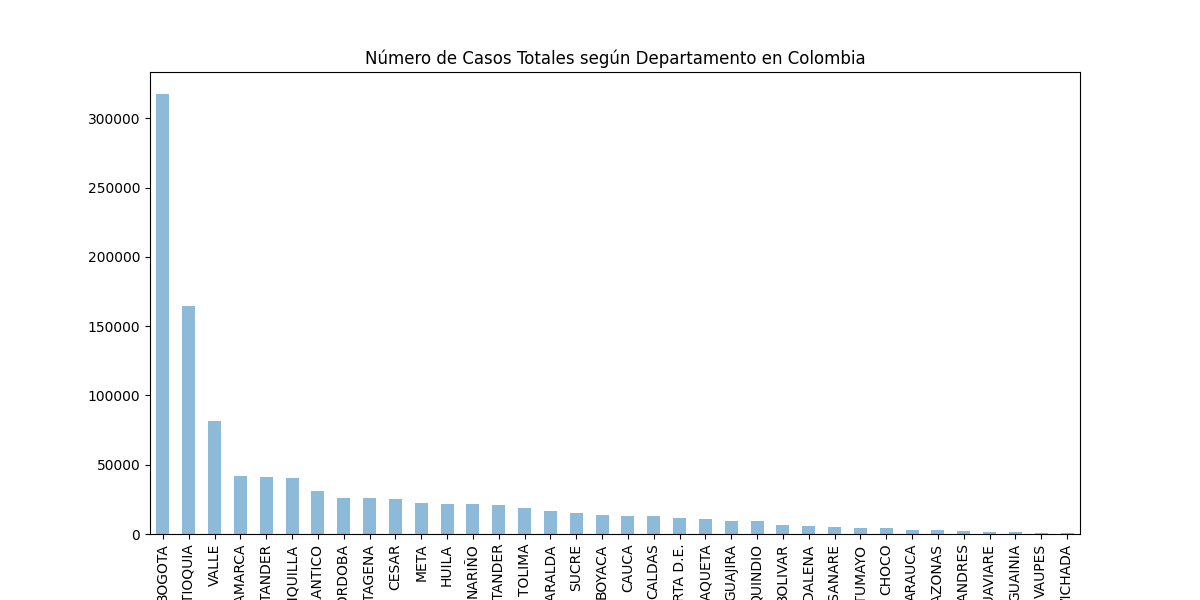
\includegraphics[width=85mm]{Figures/Figure_1.png}}
\subfigure[\scriptsize Gráfica Número de Casos según el Sexo en Colombia]{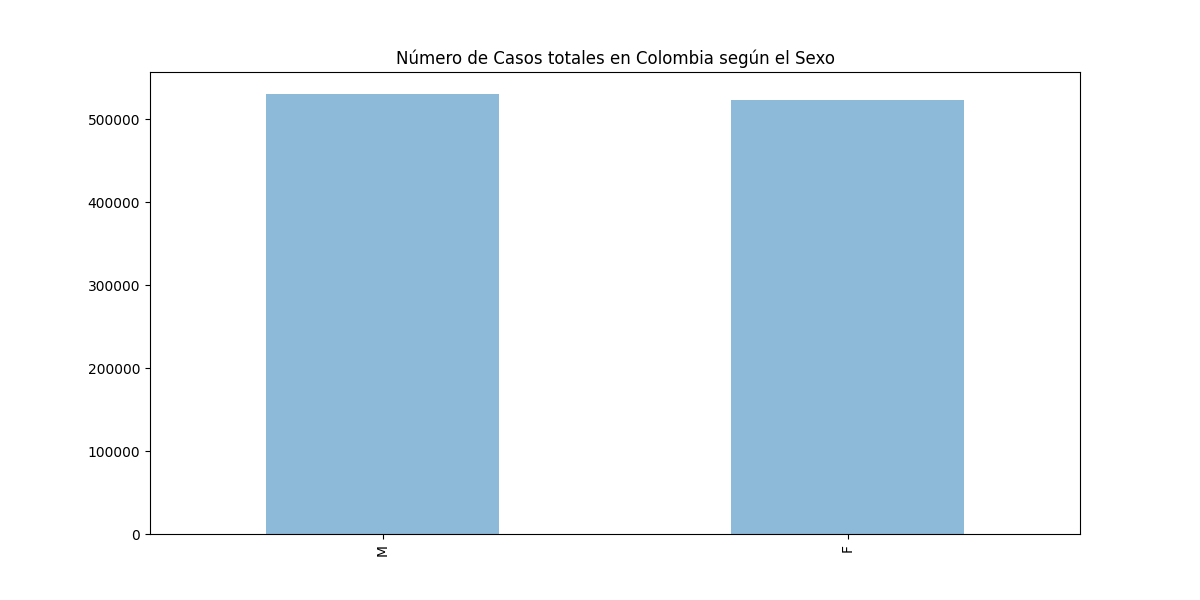
\includegraphics[width=85mm]{Figures/Figure_2.png}}
\label{fig:lego}
\end{figure}

\begin{figure}[htbp]
\centering
\subfigure[\scriptsize Gráfica Número de Casos Recuperados en Colombia]{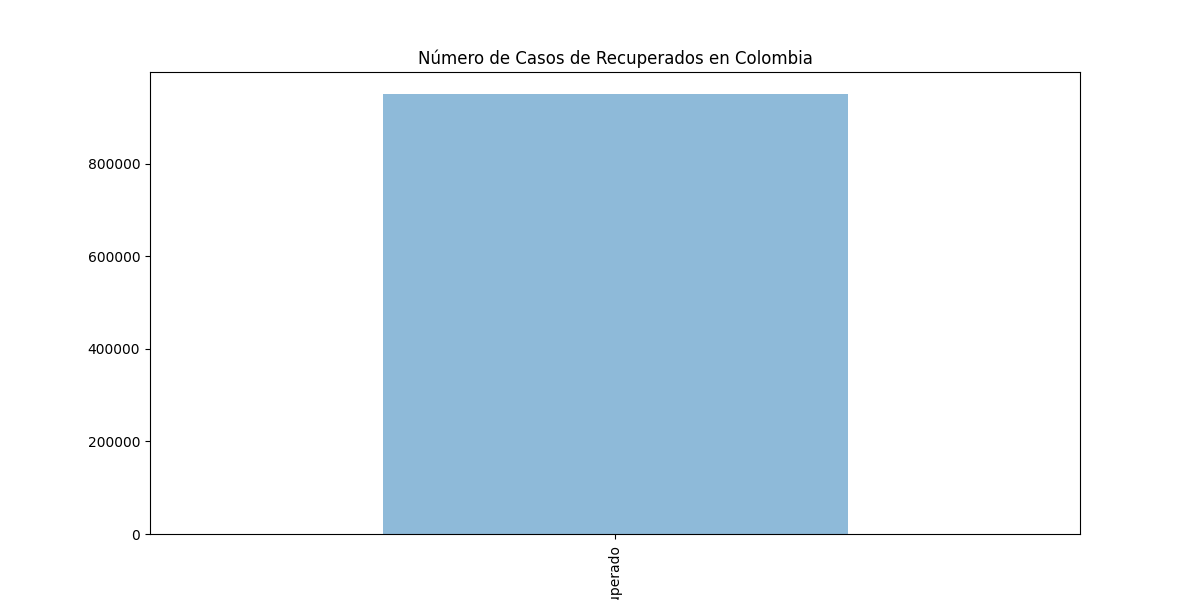
\includegraphics[width=80mm]{Figures/Figure_3.png}}
\subfigure[\scriptsize Gráfica Número de Casos Fallecidos en Colombia]{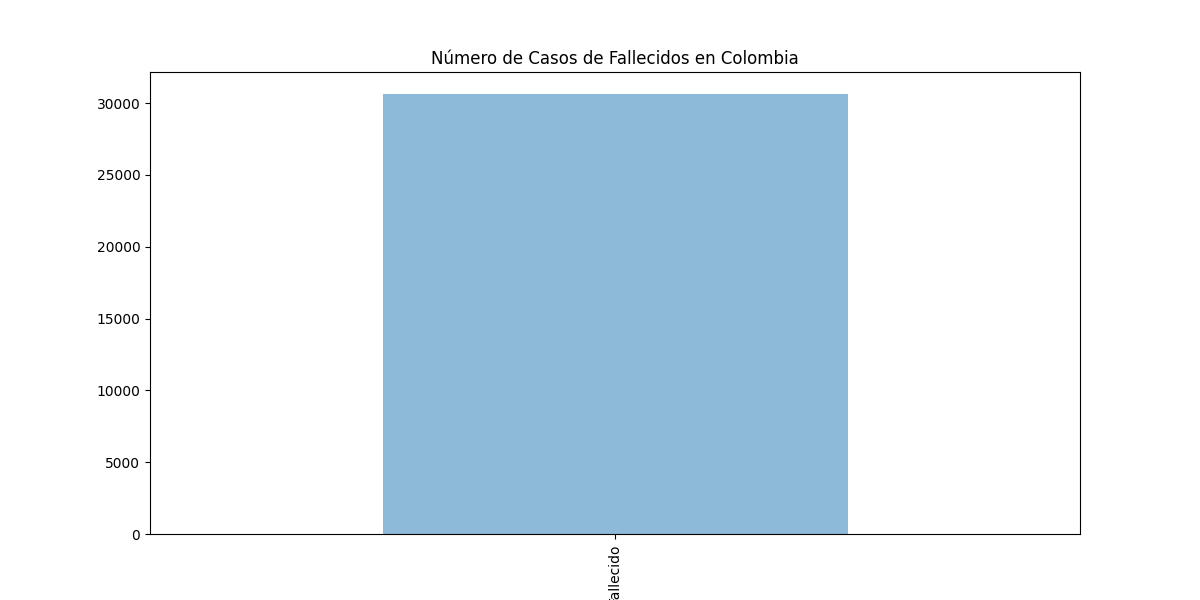
\includegraphics[width=80mm]{Figures/Figure_4.png}}
\caption{ Gráficas en estilo de Barras Verticales} \label{fig:lego}
\end{figure}
\\\

\begin{figure}[htbp]
\centering
\subfigure[\scriptsize Gráfica Porcentajes de Casos Según el Sexo ]{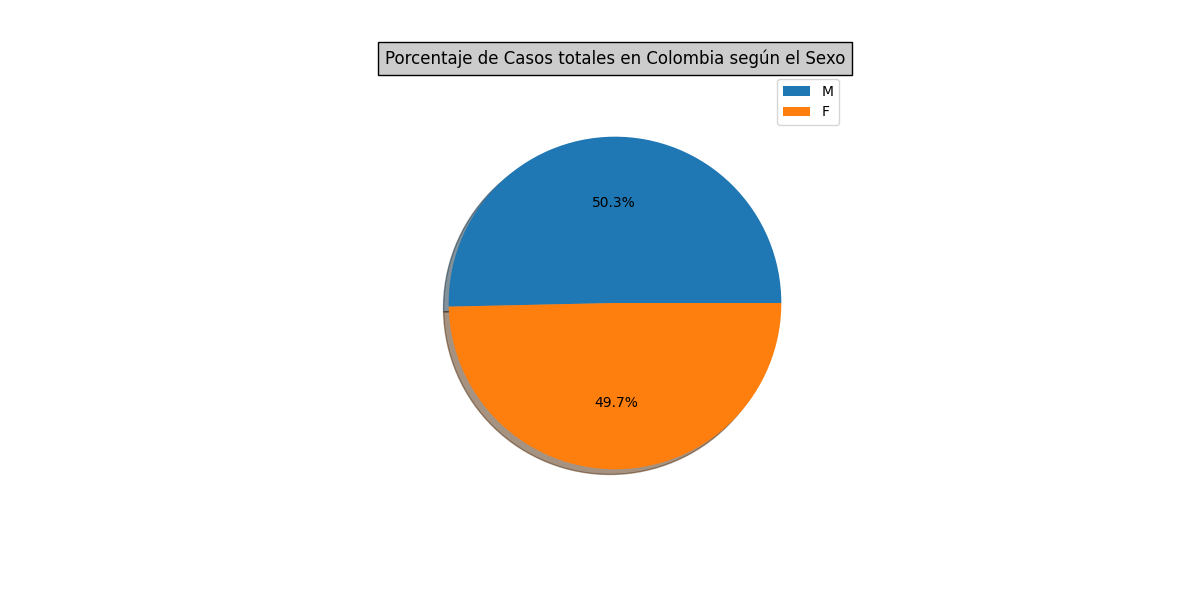
\includegraphics[width=80mm]{Figures/Figure_5.png}}
\subfigure[\scriptsize Gráfica Porcentajes de Casos Según su situación]{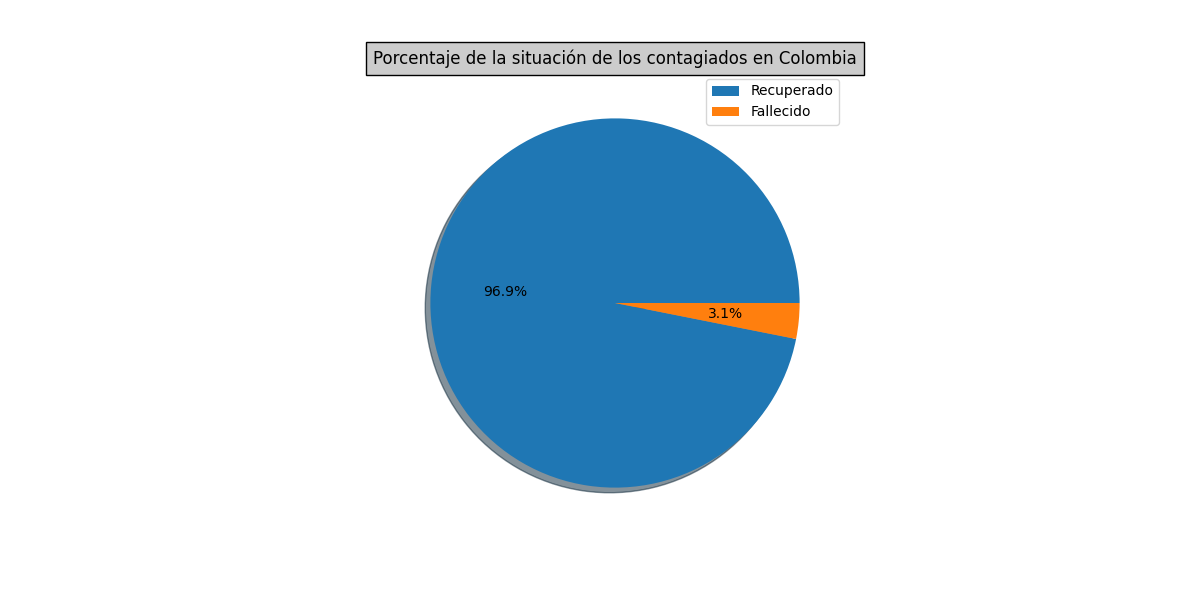
\includegraphics[width=80mm]{Figures/Figure_6.png}}
\caption{ Gráficas en estilo de Torta} \label{fig:lego}
\end{figure}
\\\
\\\
\\\
\\\
\\\
\\\
\\\
\\\
\\\

Finalmente, se añade el código para ejecutar el mapa de calor de Colombia. Para esto se utilizó un enlace externo donde están los datos GeoJson con los polígonos de cada Departamento.De hecho, se utilizó la librería  "plotly.express" la cual nos permitió crear el mapa teniendo en cuenta el archivo GeoJson y el archivo CSV.
\\\

\begin{lstlisting}
#//////////////////MAPA DE CALOR COLOMBIA//////////////////////////
repo_url = 'https://gist.githubusercontent.com/john-guerra/43c7656821069d00dcbc/raw/be6a6e239cd5b5b803c6e...
7c2ec405b793a9064dd/Colombia.geo.json' #Archivo GeoJSON
mx_regions_geo = requests.get(repo_url).json()
extra=np.array(data.Departamento.value_counts())
casosDepartamentos=np.array([extra[1],extra[6],extra[0],extra[24],extra[17],extra[19],extra[21]...
,extra[18],extra[9],extra[7],extra[3],extra[28],extra[12],extra[22],extra[25],extra[10],extra[11]...
,extra[13],extra[23],extra[15],extra[4],extra[16],extra[14],extra[2],extra[29],extra[26],extra[27]...
,extra[30],extra[33],extra[32],extra[34],extra[35],extra[31]])
nombresDepartamentos=np.array(["ANTIOQUIA", "ATLANTICO", "SANTAFE DE BOGOTA D.C", "BOLIVAR", "BOYACA", "CALDAS", "CAQUETA", "CAUCA", "CESAR", "CORDOBA", "CUNDINAMARCA", "CHOCO", "HUILA", "LA GUAJIRA", "MAGDALENA", "META", "NARIÑO", "NORTE DE SANTANDER", "QUINDIO", "RISARALDA", "SANTANDER", "SUCRE", "TOLIMA", "VALLE DEL CAUCA", "ARAUCA", "CASANARE", "PUTUMAYO", "AMAZONAS", "GUAINIA", "GUAVIARE", "VAUPES", "VICHADA", "ARCHIPIELAGO DE SAN ANDRES PROVIDENCIA Y SANTA CATALINA"])

fig = px.choropleth(data_frame=data,
                    geojson=mx_regions_geo,
                    locations=nombresDepartamentos, # nombre de la columna del Dataframe
                    featureidkey='properties.NOMBRE_DPT',  # ruta al campo del archivo GeoJSON con el que se hará la relación (nombre de los estados)

                    color=casosDepartamentos, #El color depende de las cantidades
                    color_continuous_scale="burg", #greens
                    #scope="north america"
                   )

fig.update_geos(showcountries=False, showcoastlines=False, showland=False, fitbounds="locations")

fig.update_layout(
    title_text = 'Casos de infección en Colombia',
    font=dict(
        #family="Courier New, monospace",
        family="Ubuntu",
        size=18,
        color="#7f7f7f"
    )
)
plotly.offline.plot(fig)

\end{lstlisting}
\\\

Entregándonos la siguiente gráfica:
\\\

\begin{figure}[htbp]
\centering
\subfigure[\scriptsize ]{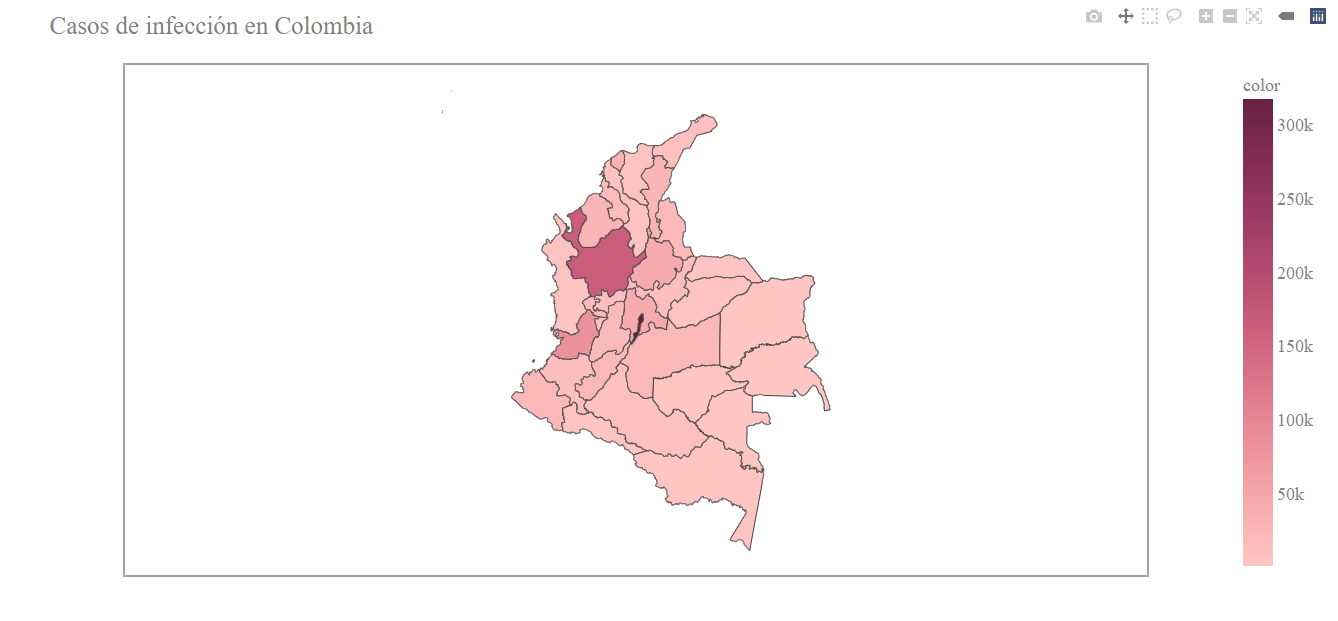
\includegraphics[width=90mm]{Figures/Figure_7.png}}
\caption{ Mapa de Calor Colombia} \label{fig:lego}
\end{figure}
\\\

\textbf{CÓDIGO PARA DATOS COVID BOGOTÁ}
\\\

Para el caso de Bogotá  se abre el archivo CSV local y se obtienen todos los datos. Además, se hace el arreglo de los nombres de las columnas, se elimina la primera fila que no entrega información relevante y se establece los rangos de edad que se tendrán en cuenta en las gráficas.
\\\

\begin{lstlisting}
#///////////////////BOGOTÁ//////////////////////////////////////
#Abrir el CSV que se descargó de Bogotá y obtener la información

dato =pd.read_csv('Archivo/DataBogota.csv', delimiter=";", encoding='iso-8859-1',names=['Fecha_Sintomas', 'FechaDiagnostico', 'Ciudad', 'Localidad', 'Edad', 'Uni_Med', 'Sexo', 'Fuente_Contagio', 'Ubicacion', 'Estado'])
dato.head()
dato=dato.drop([0], axis=0) #Borrar la primera fila que tiene texto innecesario
dato.Edad=dato.Edad.astype(float) #Convertir la columna Edad a float
age_groups = pd.cut(dato.Edad, bins=[19, 40, 65, np.inf]) #Rangos de edad
\end{lstlisting}
\\\

Después se realiza el código para crear las 6 gráficas de Barras, las 2 gráficas de Tortas y las 3 gráficas de área, en donde se busca representar los datos sobre los Localidades, Sexo, Recuperados, Fallecidos, Edad y según su condición.
\\\

\begin{lstlisting}

#GRÁFICAS DE BARRAS

fig=plt.figure(figsize=(12,6))
dato.Sexo[dato.Sexo != "SEXO"].value_counts().plot(kind='bar', alpha=0.5)
plt.title('Número de Casos totales en Bogotá según el Sexo')
plt.show()

fig2=plt.figure(figsize=(12,6))
dato.Estado[dato.Estado == "Recuperado"].value_counts().plot(kind='bar', alpha=0.5)
plt.title('Número de Casos de Recuperados en Bogotá')
plt.show()

fig3=plt.figure(figsize=(12,6))
dato.Estado[dato.Estado == "Fallecido"].value_counts().plot(kind='bar', alpha=0.5)
plt.title('Número de Casos de Fallecidos en Bogotá')
plt.show()

fig1=plt.figure(figsize=(12,6))
dato.Localidad[dato.Localidad != "Sin dato"].value_counts().plot(kind='bar', alpha=0.5)
plt.title('Número de Casos Totales según Localidad en Bogotá')
plt.show()

fig1=plt.figure(figsize=(12,6))
pd.crosstab(dato.Localidad[dato.Localidad != "Sin dato"], dato['Sexo']).plot(kind='bar', alpha=0.5)
plt.title('Número de Casos totales en Bogotá según el Sexo y la Localidad')
plt.show()

fig1=plt.figure(figsize=(12,6))
pd.crosstab(dato.Localidad[dato.Localidad != "Sin dato"], age_groups).plot(kind='bar', alpha=0.5)
plt.title('Número de Casos totales en Bogotá según el rango de edad y la Localidad')
plt.show()

#GRÁFICAS DE TORTAS
fig1=plt.figure(figsize=(12,6))
plt.pie(dato.Sexo[dato.Sexo != "SEXO"].value_counts(), autopct="%1.1f%%", shadow=True, radius= .9)
plt.title('Porcentaje de Casos totales en Bogotá según el Sexo', bbox={"facecolor":"0.8","pad":5})
plt.legend( labels= dato.Sexo.value_counts().index.unique(), loc='upper right')
plt.show()

fig1=plt.figure(figsize=(12,6))
plt.pie(dato.Estado[dato.Estado != "ESTADO"].value_counts(), autopct="%1.1f%%", shadow=True, radius= .999)
plt.title('Porcentaje de la situación de los contagiados en Bogotá', bbox={"facecolor":"0.8","pad":5})
plt.legend( labels=['%s, %1.1f%%' % (
        l, (float(s) / len(dato)) * 100) for l, s in zip(dato.Estado.value_counts().index.unique(), dato.Estado.value_counts())], loc='upper right')
plt.show()

#GRÁFICAS EXTRAS BOGOTÁ

fig1=plt.figure(figsize=(12,6))
dato.Localidad[dato.Localidad != "Sin dato"].value_counts().plot(kind='area', alpha=0.5)
plt.title('Número de Casos Totales según Localidad en Bogotá')
plt.show()

fig1=plt.figure(figsize=(12,6))
pd.crosstab(dato.Localidad[dato.Localidad != "Sin dato"], dato['Sexo']).plot(kind='area', alpha=0.5)
plt.title('Número de Casos totales en Bogotá según el Sexo y la Localidad')
plt.show()

fig1=plt.figure(figsize=(12,6))
pd.crosstab(dato.Localidad[dato.Localidad != "Sin dato"], age_groups).plot(kind='area', alpha=0.5)
plt.title('Número de Casos totales en Bogotá según el rango de edad y la Localidad')
plt.show()
\end{lstlisting}
\\\

Al ejecutar todo el código se obtienen las siguientes gráficas:
\\\

\begin{figure}[htbp]
\centering
\subfigure[\scriptsize Gráfica Número de Casos Totales según el Sexo en Bogotá]{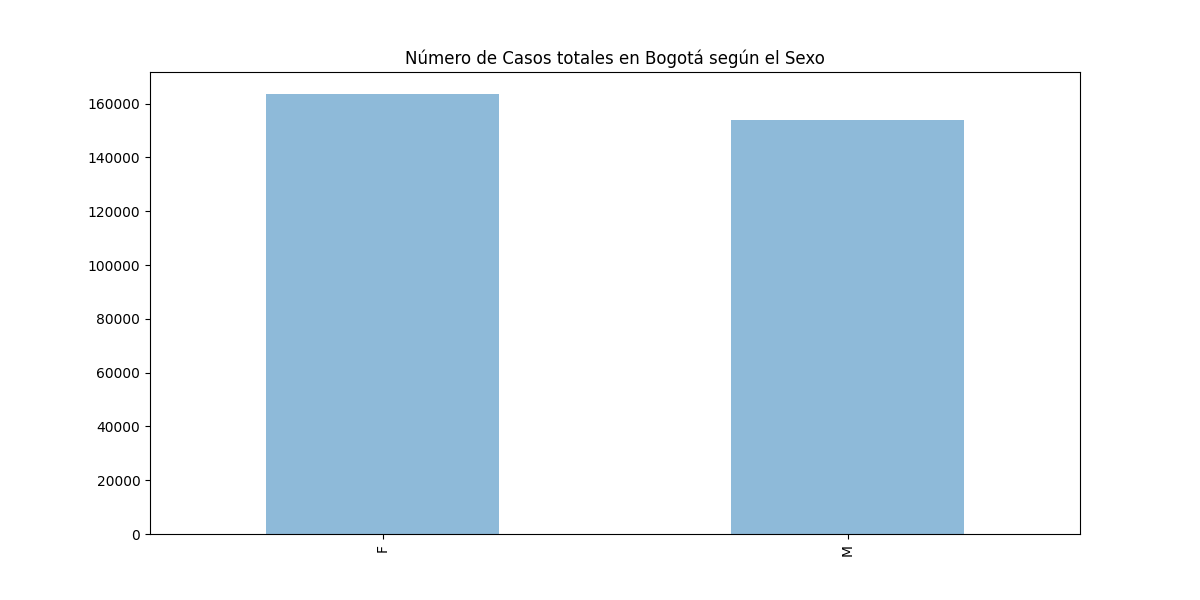
\includegraphics[width=60mm]{Figures/1Figure_1.png}}
\subfigure[\scriptsize Gráfica Número de Casos Recuperados en Bogotá Colombia]{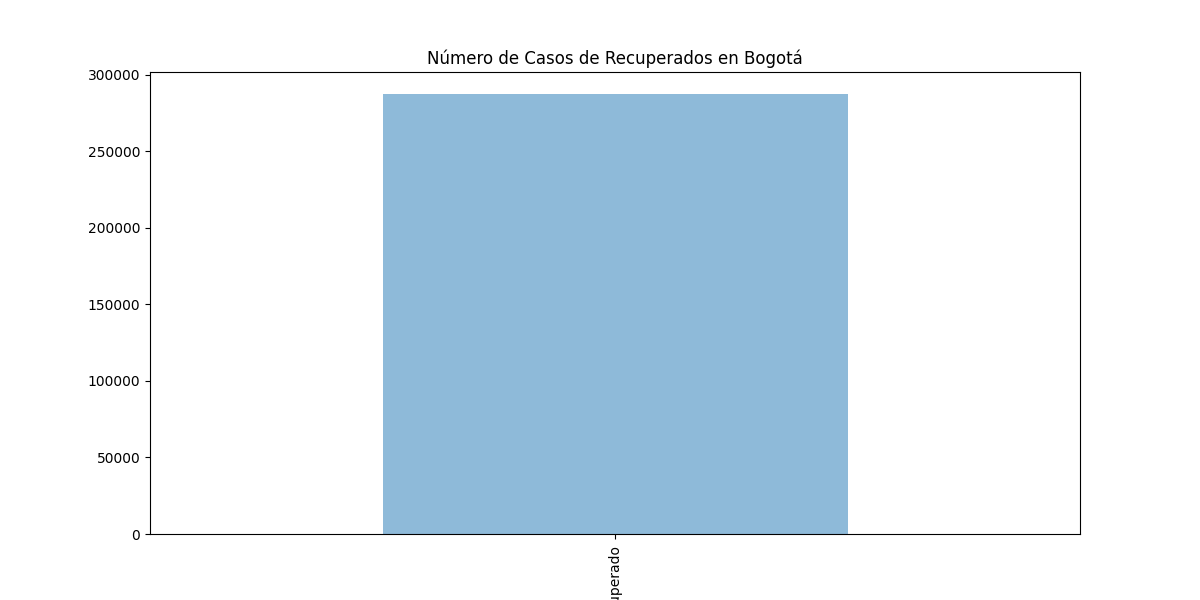
\includegraphics[width=60mm]{Figures/1Figure_2.png}}
\label{fig:lego}
\end{figure}

\begin{figure}[htbp]
\centering
\subfigure[\scriptsize Gráfica Número de Fallecidos en Bogotá]{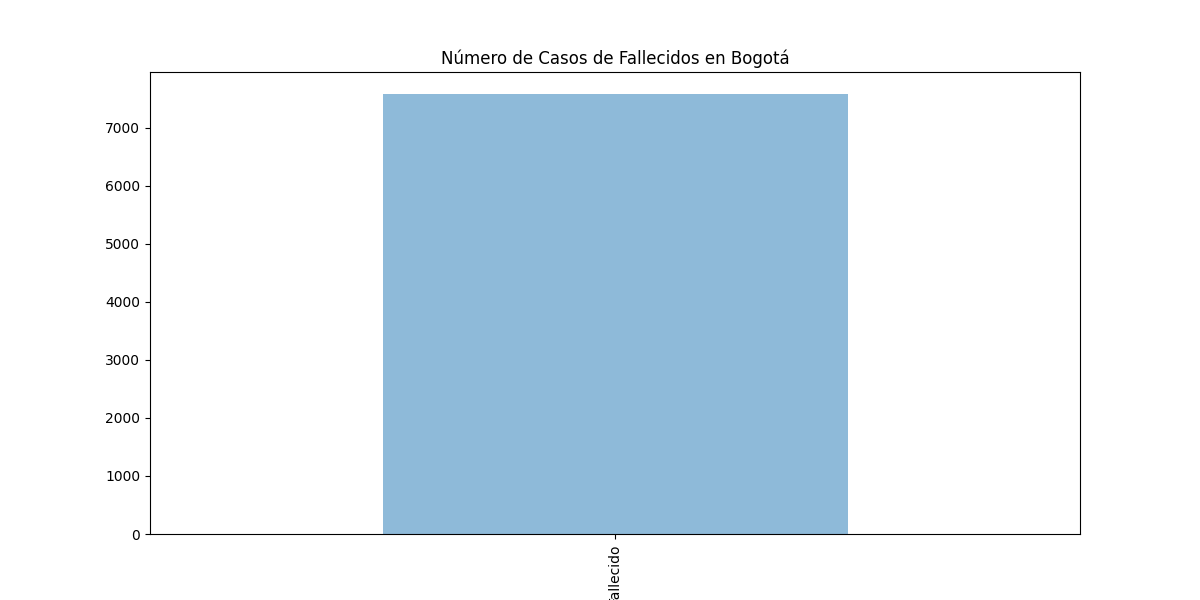
\includegraphics[width=75mm]{Figures/1Figure_3.png}}
\subfigure[\scriptsize Gráfica Número de Casos Totales según la Localidad en Bogotá]{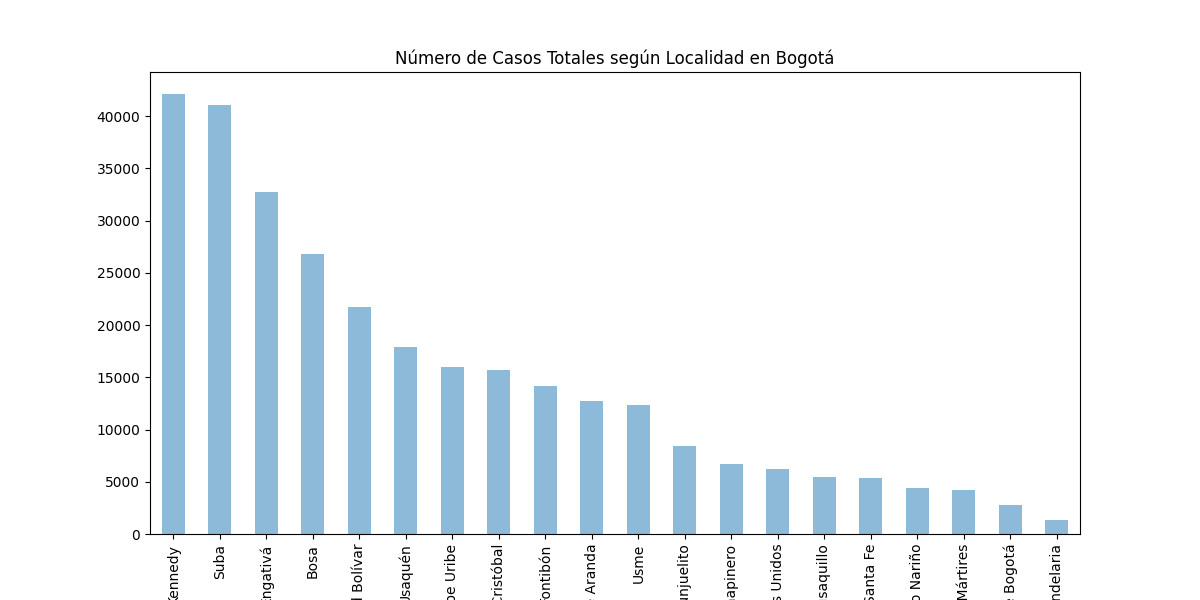
\includegraphics[width=75mm]{Figures/1Figure_4.png}}
\subfigure[\scriptsize Gráfica Número de Casos Totales en Bogotá según el Sexo y la Localidad]{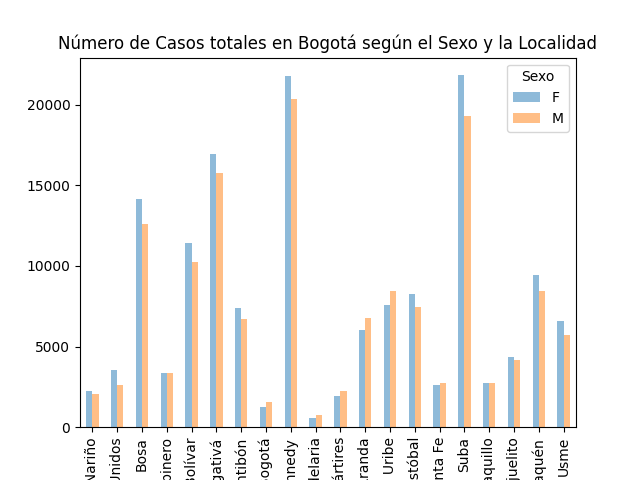
\includegraphics[width=75mm]{Figures/1Figure_5.png}}
\subfigure[\scriptsize Gráfica Número de Casos Totales en Bogotá según la Edad y la Localidad]{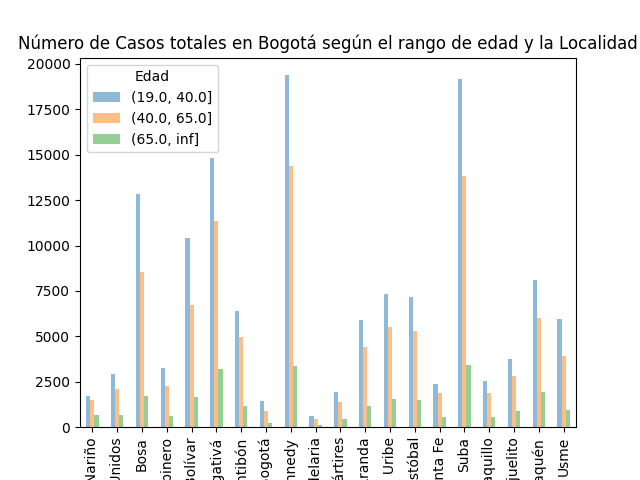
\includegraphics[width=75mm]{Figures/1Figure_6.png}}
\caption{ Gráficas en estilo de Barras Verticales} \label{fig:lego}
\end{figure}
\\\

\begin{figure}[htbp]
\centering
\subfigure[\scriptsize Gráfica Porcentajes de Casos Según el Sexo en Bogotá ]{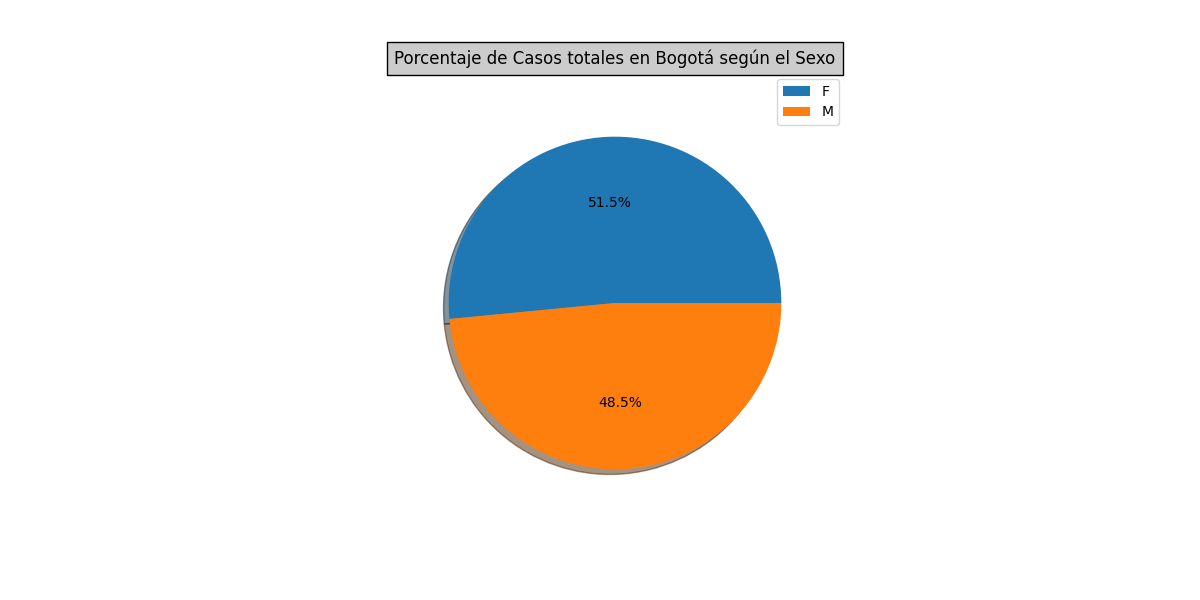
\includegraphics[width=82mm]{Figures/1Figure_7.png}}
\subfigure[\scriptsize Gráfica Porcentajes de Casos Según su situación en Bogotá]{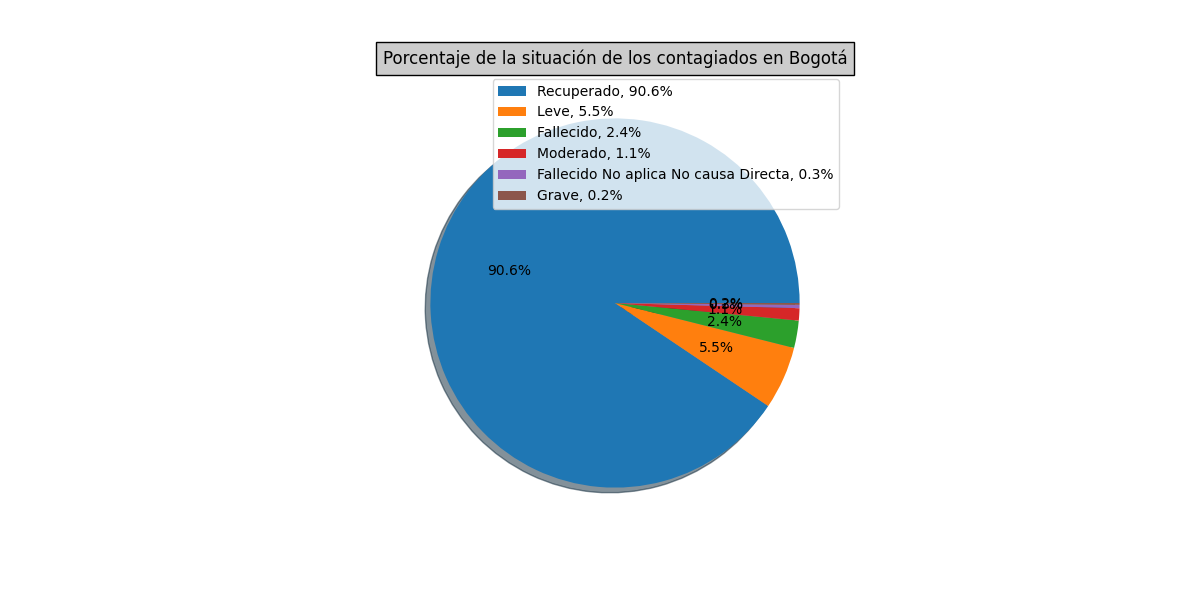
\includegraphics[width=82mm]{Figures/1Figure_8.png}}
\caption{ Gráficas en estilo de Torta} \label{fig:lego}
\end{figure}
\\\

\begin{figure}[htbp]
\centering
\subfigure[\scriptsize Número de Casos Totales Según la Localidad en Bogotá ]{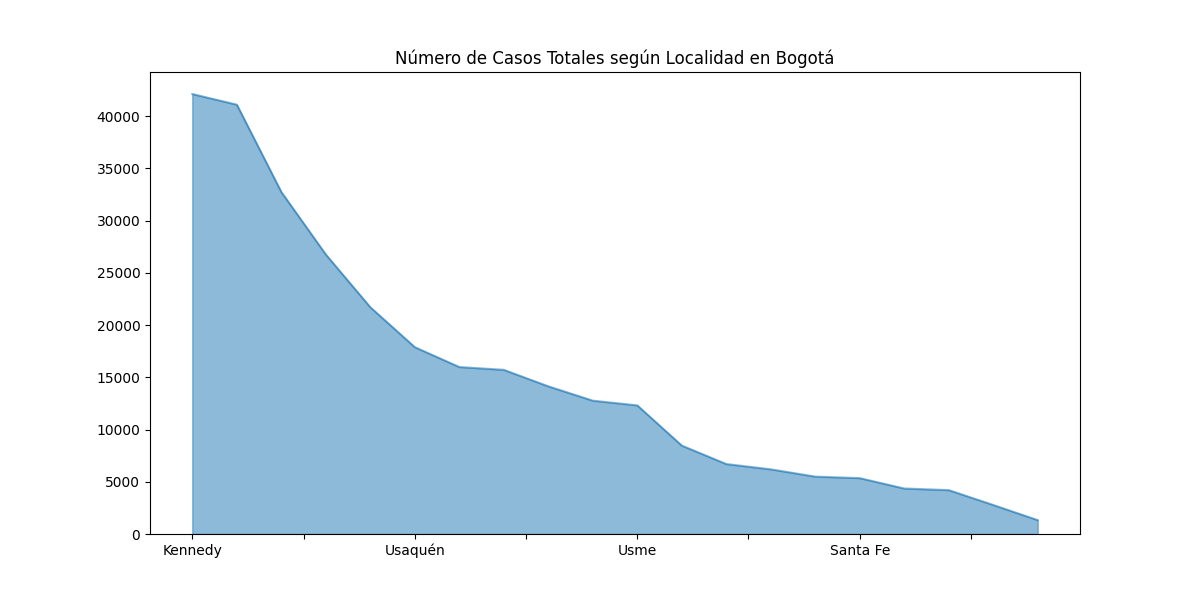
\includegraphics[width=70mm]{Figures/1Figure_9.png}}
\subfigure[\scriptsize Número de Casos Totales Según la Localidad y el Sexo en Bogotá]{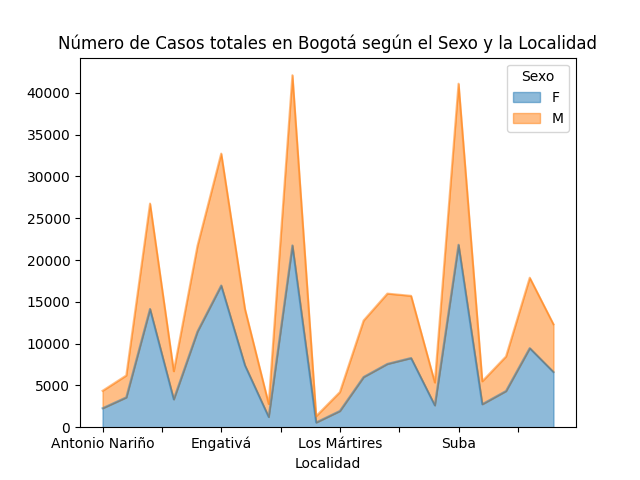
\includegraphics[width=50mm]{Figures/1Figure_10.png}}
\subfigure[\scriptsize Número de Casos Totales Según la Localidad y la Edad en Bogotá]{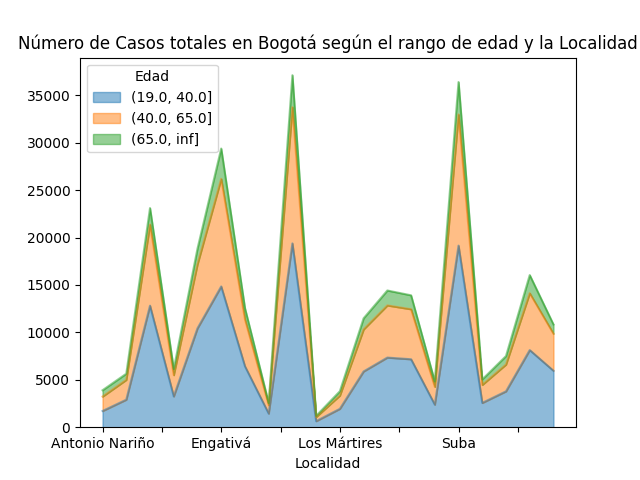
\includegraphics[width=50mm]{Figures/1Figure_11.png}}
\caption{ Gráficas en estilo Área} \label{fig:lego}
\end{figure}
\\\
\\\
\\\
\\\
\\\

Finalmente, se añade el código para ejecutar el mapa de calor de Bogotá. Para esto se utilizó un enlace externo donde están los datos GeoJson con los polígonos de cada localidad.De hecho, se utilizó la librería  "plotly.express" la cual nos permitió crear el mapa teniendo en cuenta el archivo GeoJson y el archivo CSV.
\\\

\begin{lstlisting}

#//////////////////MAPA DE CALOR BOGOTÁ//////////////////////////
repo_url2 = 'https://raw.githubusercontent.com/JessicaParrado/Localidades/main/bogota_localidades.geojson' #Archivo GeoJSON
bo_regions_geo = requests.get(repo_url2).json()
extra2=np.array(dato['Localidad'].value_counts())
casosLocalidades=np.array([extra2[4], extra2[1], extra2[7], extra2[0], extra2[11], extra2[18], extra2[16], extra2[14], extra2[9], extra2[2], extra2[20], extra2[13], extra2[5], extra2[15], 1345, extra2[8], extra2[6], extra2[12], extra2[3], extra2[10]])
nombresLocalidades=np.array(["CIUDAD BOLIVAR","SUBA", "RAFAEL URIBE URIBE", "KENNEDY", "USME", "LOS MARTIRES", "SANTA FE", "BARRIOS UNIDOS", "FONTIBON", "ENGATIVA", "CANDELARIA", "CHAPINERO", "ANTONIO", "TEUSAQUILLO", "SUMAPAZ", "SAN CRISTOBAL", "USAQUEN", "TUNJUELITO", "BOSA", "PUENTE ARANDA"])

fig = px.choropleth(data_frame=dato,
                    geojson=bo_regions_geo,
                    locations=nombresLocalidades, # nombre de la columna del Dataframe
                    featureidkey='properties.NOMBRE',  # ruta al campo del archivo GeoJSON con el que se hará la relación (nombre de los estados)

                    color=casosLocalidades, #El color depende de las cantidades
                    color_continuous_scale="Teal", #greens
                    #scope="north america"
                   )

fig.update_geos(showcountries=True, showcoastlines=True, showland=True, fitbounds="locations")

fig.update_layout(
    title_text = 'Casos de infección en Bogotá',
    font=dict(
        #family="Courier New, monospace",
        family="Ubuntu",
        size=18,
        color="#7f7f7f"
    )
)
plotly.offline.plot(fig)
\end{lstlisting}
\\\

Entregándonos la siguiente gráfica:
\\\

\begin{figure}[htbp]
\centering
\subfigure[\scriptsize Mapa de Calor de Bogotá]{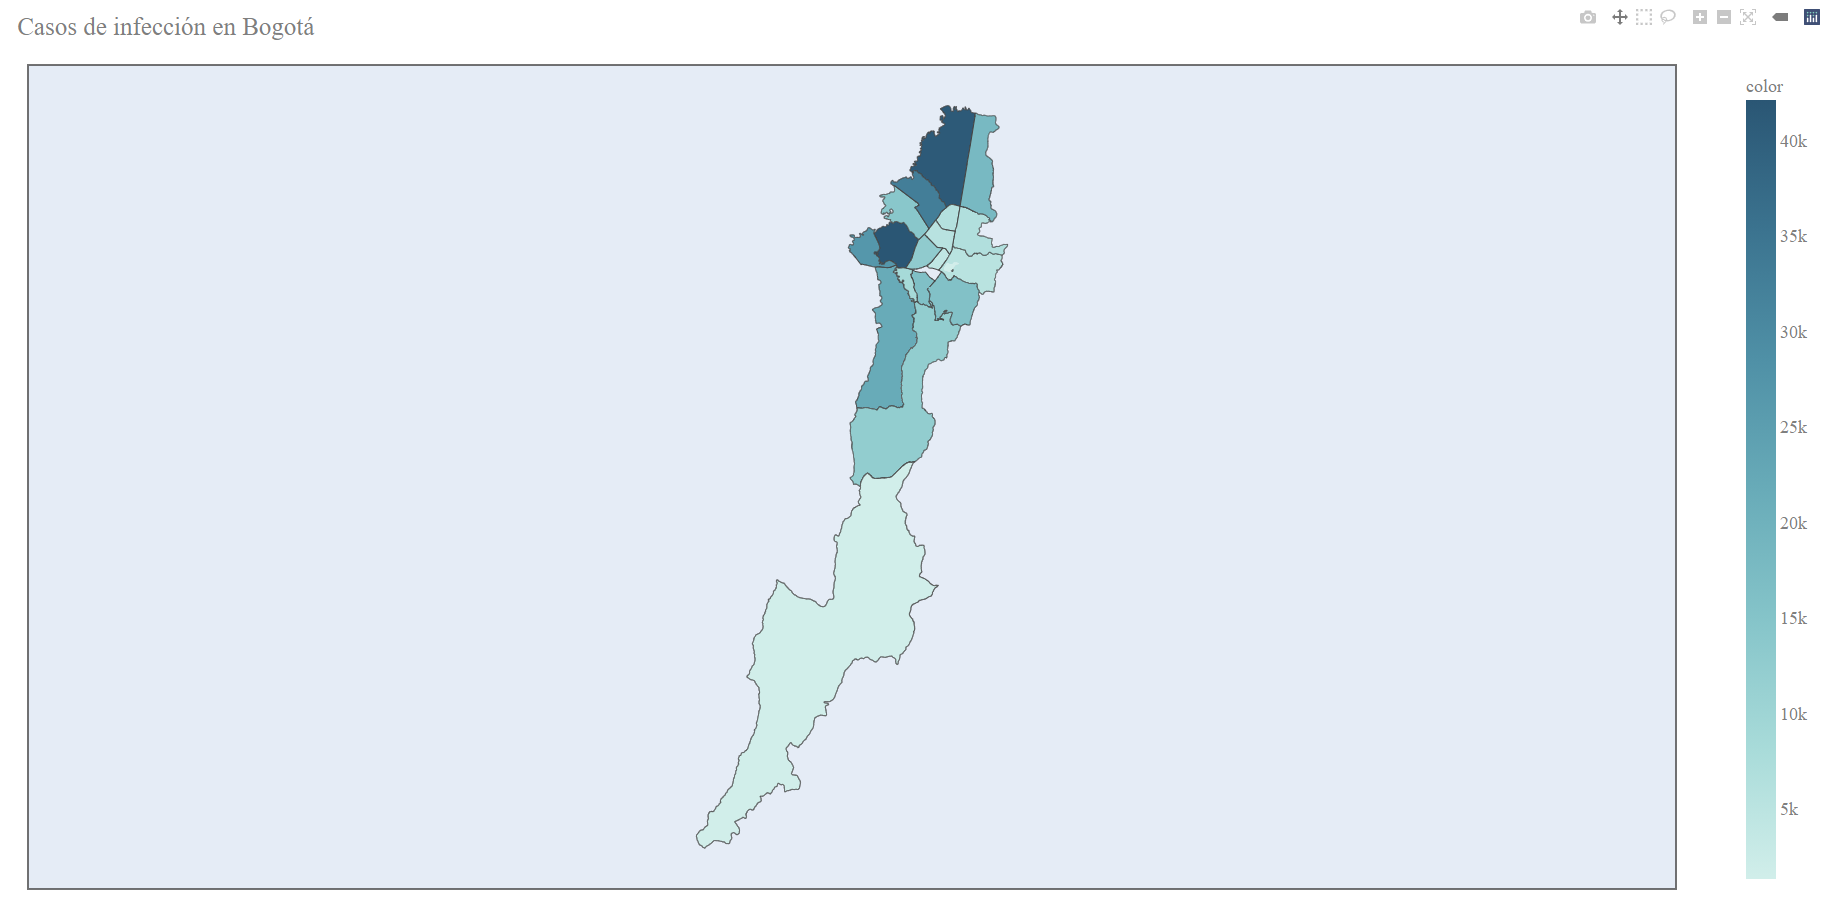
\includegraphics[width=90mm]{Figures/1Figure_12.png}}
\label{fig:lego}
\end{figure}
\\\

\section{Conclusiones}
\label{sec:conclusions}
% Escriba su texto aquí
Este año (2020) ha llegado con muchos problemas para la sociedad de todo el mundo, la pandemia ha afectado en todos los ámbitos a las personas, por ese motivo es tan importante esta información, gracias a esto, se han podido tener planes para poder solventar esta problemática de la mejor manera, acá es cuando notamos la gran importancia de la obtención, filtración, y representación de la información. Para poder lograr esto, encontramos la información necesaria que nos dio las herramientas para poder extraer los datos, a su vez este proyecto nos ayudó a entender como poder normalizar la información para hacer un uso eficaz y poder presentar información según las necesidades actuales, todo esto con el objetivo de ser eficientes a la hora de actuar frente a esta enfermedad.
\\\

\section{Repositorio Git}
\label{sec:Repositorio}

El link del repositorio git donde está el código y los documentos es el siguiente:
\\\

https://github.com/JessicaParrado/ProyectoSenialesCorte2
\\\

\\\
\nocite{*}
\bibliographystyle{IEEEtran}
\label{sec:biblio}
% Descomente y modiffique el archivo biblio.bib para agregar bibliografía
\bibliography{bib/biblio} 





%\pagestyle{empty}
\end{document}


